\section{Introduction}
\label{sec:intro}

% %!TEX root = ../../main.tex
\begin{figure}[t]
    \centering 
    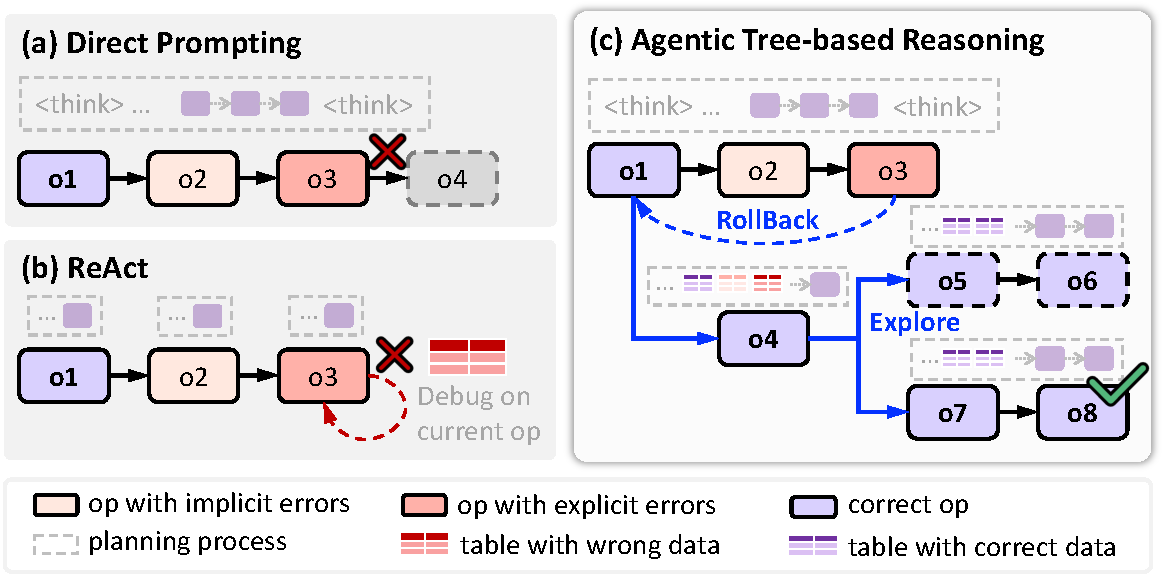
\includegraphics[width=0.99\columnwidth]{figures/fig/prompting_methods.pdf}
    % \vspace{-1em}
    \caption{Comparison of Different Inference Engine.
    }
    \label{fig:prompting_methods}
    % \vspace{-1em}
\end{figure}
%!TEX root = ../../main.tex
\begin{figure}[t]
    \centering 
    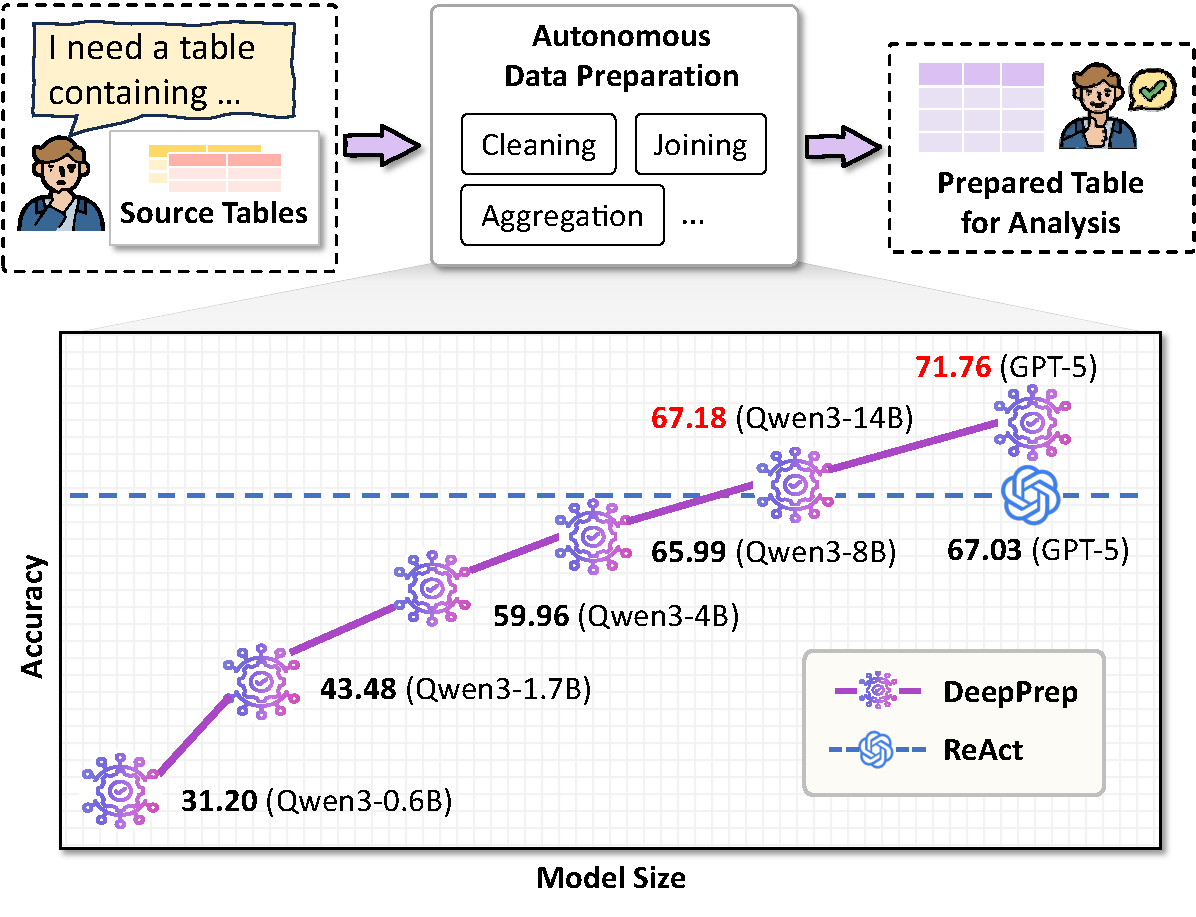
\includegraphics[width=0.85\columnwidth]{figures/fig/introduction_experiment.pdf}
    \vspace{-1em}
    \caption{Overview of Autonomous Data Preparation (Top) and Performance of \sys (Bottom).}
    \label{fig:introduction_experiment}
    \vspace{-1em}
\end{figure}
%!TEX root = ../../main.tex
\begin{figure*}[!t]
    \centering 
    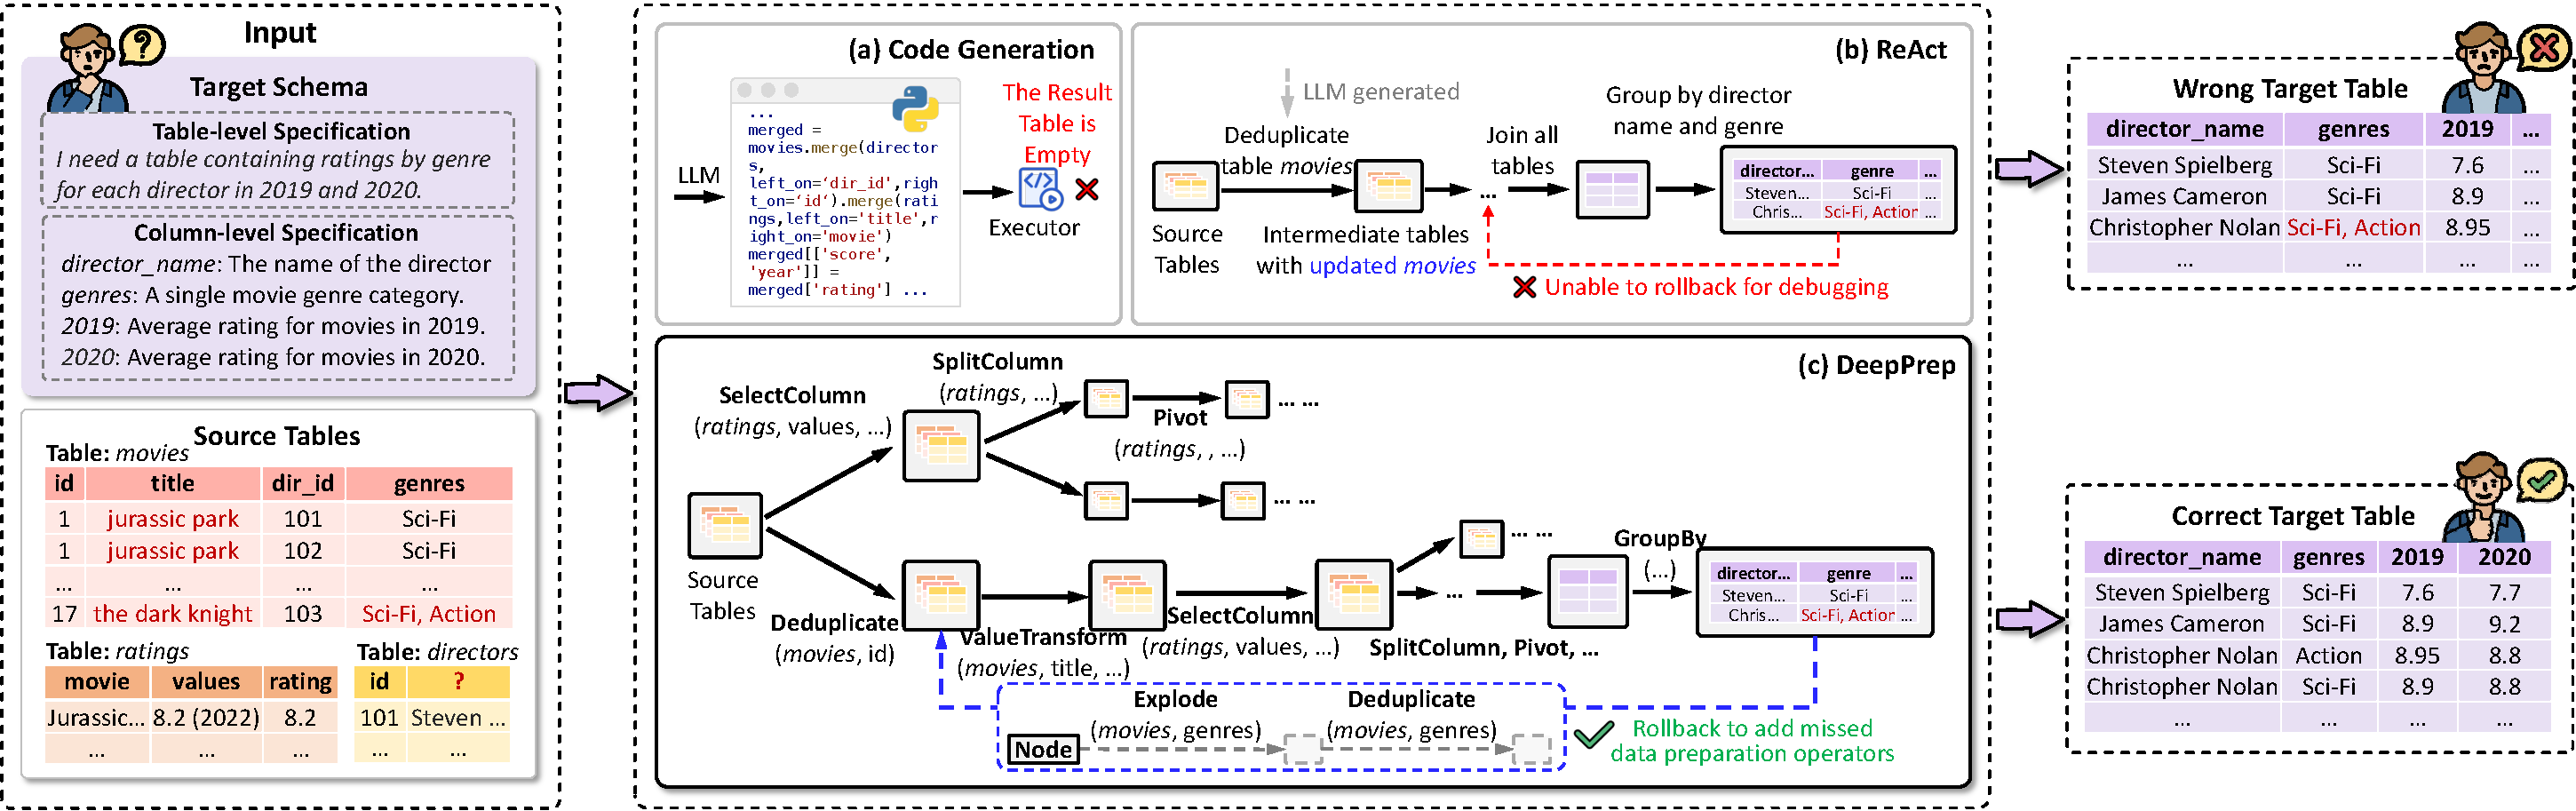
\includegraphics[width=0.95\textwidth]{figures/fig/introduction_example.pdf}
    \vspace{-1em}
    \caption{An illustrative example highlighting the core idea of \sys.
(a) Code generation makes decisions without grounding in intermediate execution results.
(b) ReAct-style approaches follow linear reasoning with limited ability to revise earlier decisions.
(c) \sys applies a tree-based structured exploration, which enables backtracking to resolve non-local errors.
    }
    \label{fig:introduction_example}
    \vspace{-1em}
\end{figure*}

Tabular Data Preparation (DP), the process of transforming raw tables into analysis-ready formats, remains a critical bottleneck in data science, often consuming 60-80\% of total analysis time~\cite{dasu2003exploratory}. 
In real-world scenarios, the ideal interaction paradigm is \textbf{Natural Language (NL) \nlwhat DP}. As illustrated in Figure~\ref{fig:introduction_experiment} (Top),
for processing heterogeneous raw tables, the users only need to provide  high-level analysis requirements (\eg \textit{``I want to analyze director performance...''}). The system should then automatically generate the necessary sequence of DP operations, ranging from data cleaning, table reconstruction and column transformation. Finally, it yields a prepared table ready for downstream analysis.

However, existing methods fail to realize this vision. Traditional tools~\cite{barowy2015flashrelate, singh2016blinkfill, he2018transform, gulwani2012spreadsheet, jin2017foofah, heer2015predictive} primarily rely on rigid specifications, \eg instance data of the target table. They fail to understand ambiguous, high-level user intent. 

Large Language Models (LLMs) bring an opportunity for NL-\nlwhat DP due to their remarkable capabilities in NL understanding and code generation. 
% Current LLM-based approaches generally fall into two categories.
A popular framework named CodeGen~\cite{sapkota2025vibe}, interactively generates and executes code (\eg Python scripts) based on DP requirements.
% While flexible, generating code for complex, recurring operations is often error-prone.
% \jie{refer to figure 1 for LLM performance} \fmh{In Figure 1, we do not report the performance of agentic codeing method}
% Moreover, the coarse granularity of code execution hinders effective debugging. 
% Moreover, CodeGen often execute multiple DP operations within one interaction without inspecting intermediate results. Thus it is difficult to pinpoint the exact step responsible for a failure.
% 这里只说一点问题就行
While flexible, generating code for complex operations is often error-prone.
Specifically, it often execute a pipeline of DP operations within one interaction without inspecting intermediate results. Thus it is difficult to pinpoint the exact step responsible for a failure when occurring bugs.

% 基于算子的方法，为了提高可控性和
\stitle{Operator-Assisted Data Preparation.}
To improve the quality of generated operation pipeline, recent frameworks~\cite{fan2024autoprep, ge2025text}
% \jie{restrict?}
constrain
the LLM to generate predefined operators. The operator, as the basic unit of pipeline, it naturally defines the granularity of intermediate result inspection.
A widely-used method named ReAct~\cite{aksitov2023rest} works in a linear way, which generates the next operator based on the result of the previous one. 
However, in DP tasks, operators are highly interdependent. A suboptimal choice at an early stage (\eg an aggressive row filter or an incorrect regex split) often manifests as a failure only several steps later. Thus, it requires to backtrack to fix early errors and explore correct path. These capabilities can not be provided by such linear method.

\stitle{The Need for Tree-Based Reasoning.}
Tree-based reasoning offers a promising solution to this challenge. It enables backtracking to previous error nodes and the exploration of multiple potential trajectories. A widely-known approach is Monte Carlo Tree Search (MCTS)~\cite{li2025alphasql, ge2025monteprep}. MCTS iteratively constructs a search tree through four phases: {selection} of promising nodes, {expansion} of new child nodes, {simulation} of outcomes, and {backpropagation} of values to update the tree.

However, MCTS relies on the \textbf{local information} during the search process, leading to \textbf{blind trial-and-error} in our task scenarios. 
Specifically, it expands new nodes based solely on the current state without referencing the historical exploration paths of other branches. So it ignores valuable failure signals from sibling nodes. Furthermore, the feedback in MCTS is typically a {scalar reward} (\eg aggregation of cumulative return and visit count in UCT~\cite{ameneyro2022towards}). Thus, the model remains unaware of the semantic cause of errors, which leads to an invalid backtracking.
% Specifically, it expands new nodes based solely on the current state without referencing the historical exploration paths of other branches, ignoring valuable failure signals from sibling nodes. Furthermore, since the feedback in MCTS is typically a scalar reward, the model remains unaware of the semantic cause of errors.

\begin{example}
    Consider the example in Figure~\ref{fig:introduction_example}. The task requires analyzing director performance across movie genres based on audience ratings from different years. It requires to perform data cleaning, table reconstruction, and column transformation operations on three source tables: ``{movies}'', ``{ratings}'', and ``{directors}''.

    Figure~\ref{fig:introduction_example}(a) illustrates the search process of MCTS for this problem. Initially, MCTS explores three sub-trees to clean the tables respectively. In the left sub-tree, after processing the table ``{ratings}'', MCTS attempts to process the table ``{movies}''. However, it focuses only on the local information of the current node and ignores previous exploration on ``{movies}''. Thus, when splitting a new node to standardize the {title} column, it repeats a previously encountered error (\eg failing to handle null values first). Furthermore, when the simulation detects an error, MCTS merely penalizes the scalar value of the current trajectory but discards the semantic information of the failure. This leads the model to select the next node based solely on global statistical value rather than correcting the current error.
    Consequently, such a blind exploration framework often requires over 50 iterations to find a correct path, which is extremely inefficient.
\end{example}

Therefore, we aim to construct a tree-based reasoning method with a global perspective to guide the exploration.
Specifically, we desire a framework that (1) is able to refer operators planned in previous branches (\textbf{global planning}) and (2) leverages previous execution results to achieve precise exploration (\textbf{global feedback}).

% utilizes \textbf{global planning} during the exploration phase, referring the operator sequences planned in previous branches and (2) leverages \textbf{global feedback}, \ie execution results rather than
% % \jie{scalars? first mention of the term without definition}
% scalar reward, to achieve precise exploration,
% % \jie{contrasting with? delete with}
% in contrast to
% the blind trial-and-error of MCTS.

\stitle{Agentic Tree-based Reasoning.}\fmh{cite some papers in the content.}
In this paper, we propose an agentic tree-based reasoning framework named \sys. We define the state of the agent as the collection of historical planning and environment interaction. This state is formulated in a tree structure, denoted as ``state tree''. Based on it, the agent iteratively uses three actions to automatically update the state and automatically conduct DP operations.
Specifically,
% \jie{In abstract, Global State Tree is capitalized. Be consistent.} \fmh{Abstract is not ready.}
in each step, \sys first employs {<analyze} to evaluate the state tree and provide a clear plan for the next step. Based on this plan, \sys uses {<expand} to extend a new branch of operators from a specific node. An external executor then executes the new branch and returns interaction results via {<execute}, which are updated into the state tree. Through this automated process, \sys generates an operator tree capable of producing the correct target table. It finally extracts the correct operator chains via {<solution} for the final output.

Specifically, we provide an example to illustrates how \sys leverages the global information to implement precise tree-based search.

\begin{example}
\label{exam:agentic_tree_based_reasoning}

    % \jie{reflection of several operators in one step is unclear in the figure}
    % \jie{operator in line flows instead of several s turns.}
    % \fmh{I think that introduction only needs to highlight the significance of tree-based reasoning. The feature that "operator in line flows instead of several turns" is specifica implementation of sys, which is better to be described in other sections.}
    Figure~\ref{fig:introduction_example}(b) demonstrates the workflow of \sys.
    % Initially, with only a start node, the model uses {<analyze} to examine the input tables and DP requirements, devising a divide-and-conquer strategy. It sequentially uses {<expand} and {<execute} to create three sub-trees for processing the distinct tables.
    Initially, starting from the root node, the model uses \texttt{<analyze} to decompose the complex requirement. It adopts a divide-and-conquer strategy, sequentially utilizing \texttt{<expand} and \texttt{<execute} to create three separate branches (sub-trees). Each branch independently performs data cleaning operations on three source tables.
    % Subsequently, as shown in the left part of Figure~\ref{fig:introduction_example}(b), \sys analyzes the global state. Although the tree contains cleaned versions of ``{movies}'', ``{ratings}'', and ``{directors}'', they initially exist on separate branches. To proceed, \sys decides to extend the ``{ratings}'' branch. Instead of starting from scratch, the model extracts the correct nodes from the history of the other two sub-trees and replicates them into the current branch during the {<expand} phase.
    Subsequently, as shown in the left part of Figure~\ref{fig:introduction_example}(b), to integrate the data, \sys decides to extend the ``{ratings}'' branch. Instead of generating new operators for the other two tables from scratch, \sys inspects the state tree (which contains three sub-trees named ``ops on ratings/movies/directors''). It identifies that valid cleaning operator sequence for ``{movies}'' and ``{directors}'' have already been successfully planned in the sibling branches. Consequently, \sys retrieves these correct nodes and replicates them into the current ``{ratings}'' branch. 
    % Subsequently, as shown in the left part of Figure~\ref{fig:introduction_example}(b), \sys analyzes the global state. Although the tree contains cleaned versions of \jie{all three tables? unclear reference. which nodes at which step}, they \jie{exist?} on separate branches. \jie{In step 2?}, sys decides to proceed from the ``{ratings}'' subtree to process ``{movies}'' and ``{directors}''. Instead of starting from scratch, the model extracts the correct nodes from the history of the other two sub-trees and replicates them into the ''{ratings}`` branch during the {<expand} phase.
    Finally, after generating a path that joins all tables and groups by genre, \sys detects an issue in the execution result: the output contains unseparated categories like ``Sci-Fi/Action''. Unlike MCTS which might blindly discard the path, \sys analyzes the lineage of operations across the tree. It pinpoints that the earlier cleaning sequence for ``{movies}'' missed a split operation. To resolve this, \sys explicitly appends \texttt{Explode} and \texttt{Deduplicate} operators to the sequence, successfully correcting the error.

    % Finally, after generating a path that processes all three tables, \sys plans to\jie{join them and group by genre?}. However, upon analyzing the execution results, \sys detects that the output table contains multi-category cells \jie{like?such as?} ``Sci-Fi/Action''. To correct this, \sys inspects the operators and results across the entire state tree, pinpointing that the cleaning process for the ``{movies}'' table missed handling multi-label categories. Consequently, the model explicitly adds {Explode} and {Deduplicate} operators to \jie{?? operator in ?? step} resolve the issue.
\end{example}

% \bi
% \item \textbf{Task-Level Divide-and-Conquer:} During exploration, \sys can decompose a task into subtasks completed on different branches. Since the global information is visible, \sys can effortlessly stitch together previously planned results in new rounds, reducing task complexity and increasing success rates. In contrast, MCTS treats branches as independent, preventing the transfer of successful experience or failure lessons.

% \item \textbf{Accurate Error Correction:} Because the state tree preserves global operations and output results, when a newly expanded branch fails, the model can analyze the error from a global perspective to precisely localize the faulty node. Unlike MCTS, which only penalizes the trajectory value and loses the semantic cause of the error, \sys can utilize the semantic feedback to backtrack accurately and correct the specific node in the next round.
% \ei

% \stitle{Technical Design.} 
To address complex real-world DP scenarios, we further enhance \sys with two key techniques.

% 这里重点说通过数据集构造让我们的模型支持**多种**操作，**长序列**规划的能力，对比其他方法operator数量少，序列短
(1) \textbf{Scalable Data Synthesis.} Existing datasets focus on single DP task or only involve short sequence of DP operators, which are insufficient for training robust agents. For example, Auto-Table~\cite{DBLP:journals/pvldb/LiHYWC23} only focuses on table reconstruction and only consider cases involving one or two operators. In contrast, practical data preparation involves operators from {multiple DP tasks} including data cleaning, table reconstruction and column transformation~\cite{heer2015predictive} and often requires combining over {a dozen operators} to achieve a practical DP requirement~\cite{2011-wrangler}.
To bridge this gap, we propose a data synthesis method to synthesize DP data involving long-chain DP operations of multiple tasks. 
% , which allows for the scalable synthesis of DP data involving long-chain DP operations from multiple tasks and enables the model to learn complex DP logic. 
Specifically, the synthesized dataset involving operations of column transformation, table reconstruction and data cleaning, with operation sequence length from 1$\sim$28.

% \fmh{where the validity and quality of each trajectory are strictly guaranteed through execution-based verification.} \jie{analysis operators?quality ?}
% Specifically, we begin with collecting real data analysis requirement from public NL2SQL datasets~\cite{spider_dataset, bird_dataset}, providing several clean and well-formatted input tables and a target table generated by executing the sql query. Then, starting from the input tables, we 

(2) \textbf{Multi-Stage Policy Learning.} The complexity of the task requires \sys to be equipped with long-chain reasoning capabilities, which can not be obtained by simply fine-tuning LLMs~\cite{xie2025logic}. Moreover, although Reinforcement Learning (RL) is demonstrated to be effective to enhance long sequence reasoning capabilities, it suffers from the {sparse rewards} issue where the model fails to roll out correct trajectories during training, making it unable to learn effectively~\cite{gao2024designing}.
To overcome these challenges, we introduce a multi-stage training framework.
First, we design a {progressive cold-start curriculum} to endow the model with the ability to instruction following and initial reasoning capabilities.
Motivated by previous research that dense reward can help improve the training performance~\cite{gao2024designing}, we employ {multiturn RL with a hybrid reward mechanism}. By integrating fine-grained state evaluation with semantic feedback, our approach provides dense signals for effective RL training.

\stitle{Two Deployment Settings.} To meet real-world needs, \sys supports two flexible settings.
First, \textbf{\sysp}, is designed for {plug-and-play} scenarios where users rely on proprietary LLMs (\eg GPT-5) without training resources. As shown in Figure~\ref{fig:introduction_experiment}, by applying our agentic tree-based reasoning via prompting, \sysp significantly enhances the baseline capabilities (surpassing MCTS with GPT-5). 
Second, \textbf{\syst}, caters to scenarios requiring {open-source or private} deployment. By applying our data synthesis and multi-stage training pipeline to further enhance open-source models capabilities on DP tasks, \syst exhibits strong {scaling laws}. As shown in Figure~\ref{fig:introduction_experiment}, the performance of \syst improves consistently with model size, allowing an 8B model to achieve competitive or even better performance comparable to baselines with GPT-5.

In summary, our contributions are as follows:
\jie{new problem definition?}

    % (1) \textbf{Agentic Tree-based Reasoning Framework.}
    (1) We propose \sys, a framework leveraging a Global State Tree to maintain the full history of planning and execution, serving as a unified foundation for both prompting (\sysp) and training (\syst) paradigms.
    
    % (2) \textbf{Scalable Synthesis and Training Strategy.} 
    (2) We introduce a scalable data synthesis pipeline alongside a multi-stage policy learning method. By combining curriculum learning with reinforcement learning on the synthesized data, we effectively equip models with the capability to handle complex, long-chain DP tasks.
    
    % (3) \textbf{SOTA Performance and Scalability.} 
    (3) Extensive experiments demonstrate that \sys achieves state-of-the-art performance. \sysp outperforms GPT-5 based baselines (\eg MCTS), while \syst exhibits robust scaling laws with various model sizes.
    % , validating the effectiveness of our approach across open-source models from 0.5B to 8B parameters.

    (4) We open-source our synthesized datasets, the code for our framework, and a suite of eight trained DP agents (from 0.5B to 8B, catering for scenarios with different computing resources). We also provide an interactive demo to facilitate community testing and deployment\footnote{\url{http://10.37.113.98:8000/}}.